\documentclass[reprint]{revtex4-1}
\usepackage{epsfig,hyperref,graphics,float,amsmath}
\usepackage{microtype,setspace,siunitx,physics,epsfig,graphicx,caption}
\begin{document}
\title{PAL 30 Report Ver. December}
\date{\today}
\author{Adam Green}
\affiliation{University of Colorado at Boulder, SMRC}

\maketitle

\section*{\label{sec:intro} Introduction}
\subsubsection*{Motivation}
\subsubsection*{Chirality}
\subsubsection*{Optical Effects}

\subsection*{Previous Results}

\subsection*{Our Group's Efforts}
\subsubsection*{Shao}
\section*{Thin Film Results}

\subsection*{Calibration of Camera}
To determine if we are seeing even-odd layer switching effects, it is important
that we know the absolute number of layers in the FSF. To this end, we have two
main options: the laser and the camera. 

In my experience, it has been difficult to get the uncertainty on the laser down
for two main reasons. First, it is difficult to keep the system exactly the
same, and any jarring or bumps will call for a re-alignment of the laser. This
will mean a re-taking of the calibration date. The second is that it is
difficult to get a consistent measurement off of the black glass. Hopefully, the
camera setup will allow us to normalize and standardize our setup.

The camera can be modelled as a fairly simple photo diode, where the grey value
recorded by a pixel is given by:
\begin{multline*}
    \label{eq:model}
    g_\textrm{value} = \frac{\textrm{Num. photons}}{s} \times \textrm{Quantum
    Efficieny [volts/photon]} \\
    \times \textrm{Exposure [s]} \times \frac{2^{12}}{\textrm{Max
    Voltage}}+\textrm{Noise} 
\end{multline*}

The two things we can control is the total flux of photons and the exposure
time. Before we can use this model, we need to verify that it works. Namely, if
we change the exposure time with a constant flux, or vice versa, that we get a
straight line that goes through the origin. 
\begin{figure}[H]
    \includegraphics[width=\columnwidth]{/media/spencer/agreenhd/Adam/Store/Calibration/PhotometricsCalibration/results/analysis/Varying-Exposure-Levels-for-Different-LED-Photometrics-Calibration.pdf}
    \caption{As different photon flux is incident on the camera, the
        greyvalue-vs-exposure time has a different slope. It also looks fairly
    linear.}
\end{figure}

We can make this more qualitative by fitting lines to each of these data sets
and then visualizing how the slope and intercepts of those lines change as the
LED power is increased.
\begin{figure}[H]
    \includegraphics[width=\columnwidth]{/media/spencer/agreenhd/Adam/Store/Calibration/PhotometricsCalibration/results/analysis/slope-and-intercept-of-expvsgrey-for-each-LED.pdf}
    \caption{The slope is nicely linear. The equation of the line is given by
    $y=.20 \times x + 0.21$, and following our simple model, this means that
    $\frac{\textrm{Quantum Effiency}\times 2^{12}}{\textrm{Max Voltage}} = .2$,
    and the fact that the intercept is so small ($b=.20$) and the high degree of
    linearity of the fit shows us that the camera is behaving well over a large
range of values}
\end{figure}

As you can see, there is a constant offset. I am not clear about what would
cause this, whether it is a dark current, background light/blackbody photons,
but it isn't constant, as we can plot the slopes and intercepts and see how they
change as more light is incident. There is also no clear discernible pattern.

The saving grace is that the intercept is fairly small (180 gv compared to the
1800 gv where I will be working), so it shouldn't affect the results. Also, the
variance in the grey values of a sample are usually of the order of 200, so it
is unlikely that the noise intercept will dramatically change the results.


We can also look at a range of LED power that would mimic the light incident on
our camera from reflection from films, this is shown in Figure.
\ref{fig:smallslopes}

\begin{figure}[H]
    \includegraphics[width=\columnwidth]{/media/spencer/agreenhd/Adam/Store/Calibration/PhotometricsCalibration/results/analysis/slope-and-intercept-of-expvsgrey-for-small-LED.pdf}
    \caption{Again, a strong linear correlation. However, the equation of the
    line is different, which suggests that either something about the quantum
efficiency is changing, or my LED power is not outputting the same amount of
power. I think the second option is more likely. \label{fig:smallslopes}}
\end{figure}

As seen in Fig. \ref{fig:smallslopes}, at small light levels, the camera is
still behaving linearly, however the equation of the line is different. This can
be seen dramatically below, in Fig. \ref{fig:allslopes}.


\begin{figure}[H]
    \includegraphics[width=\columnwidth]{/media/spencer/agreenhd/Adam/Store/Calibration/PhotometricsCalibration/results/analysis/slope-and-intercept-of-expvsgrey-for-all-LED.pdf}
    \caption{This is just the two plots above plotted on the same axis. This
    is a piece of evidence to suggest that the LED source is not giving off
constant power in time. \label{fig:allslopes} It is worth noting that I took
these two sets of measurements on different days of the week.}
\end{figure}

I've verified the model of the camera, and shown that for the regimes that we
will be working in, that it is linear. Note, I have also taken a lot of data to
try to cover the parameter space of this model, and it all works fairly well.

More work should be done to verify the long term stability of the LED power
source, however, I've taken some data that shows that over small time scales,
the LED gives consistent power out, shown in Fig. \ref{fig:constant}.
\begin{figure}[H]
    \includegraphics[width=\columnwidth]{/media/spencer/agreenhd/Adam/Store/Calibration/PhotometricsCalibration/results/analysis/verifyLEDpower.pdf}
    \caption{Over an hour, the LED is giving a very steady output of power.
    \label{fig:constant}}
\end{figure}



\subsection*{Results}
In this section I will present the results that I have obtained. To date, I've
looked at three samples of PAL30. Unfortunately, I didn't get a lot of data with
the first one, the second one gave us a lot of data but the camera had yet to be
calibrated so I didn't take a black glass shot (however, we still may be able to
extract the layer step number by a cleverly fitting. It is probably unlikely,
however, as I was not making careful light measurements.)

The third run was the best so far. I had aligned the optical and rotation axis
of the scope, so now we can rotate the stage and try to detect tilt and also see
how the polarization domains change. However, I had some trouble actually
drawing the films so I was only able to look at three films in depth. They are
all stored in chronological order in this directory structure under PAL30.

Along the way, I've also developed numerous tools that will aid in our data
analysis. 
\begin{enumerate}
\item intenmap.py will plot the circumferential intensity of a point that a user
    clicks. It was made using tkinter (still needs some work to clean up)
\item rotate.py will rotate images
\item I have pretty robust tooling to automatically extract the exposure times
    and LED power of image files, which will allow us to process them more
    quickly. I am also in the process of creating a toolchain to quickly and
    easily create layer step guesses.
\end{enumerate}
\subsection*{Tilt}
We haven't seen the strongest evidence of tilt yet. 

\begin{figure}[H]
    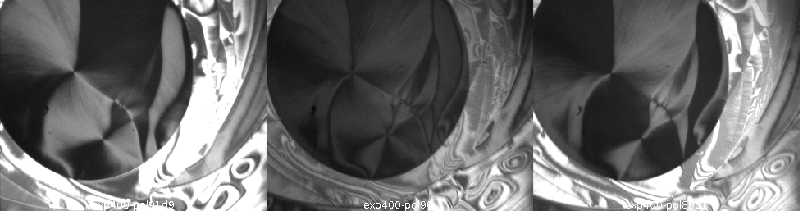
\includegraphics[width=\columnwidth]{/media/spencer/agreenhd/Adam/Store/PAL30/PAL30/4-11-2015/Presentation/Tilt/film4-T95-tiltevidence.pdf}
    \caption{Rotating the polarizer slightly through crossed\label{pic:tilt}}
\end{figure}
We can plot the circumferential intensity of the large defect in the upper left,
and the results are displayed below.

\begin{figure}[H]
    \includegraphics[width=\columnwidth]{/media/spencer/agreenhd/Adam/Store/PAL30/PAL30/4-11-2015/Presentation/Tilt/tiltevidence-film4-t95.png}
    \caption{Strong evidence for tilt would show up in asymmetries between the
    peaks at $\pi$ degrees from each other-- due to the fact that the light is
not incident perfectly normal to the plane. This is described in detail in
various thesis from the films lab.\label{fig:tilt}}
\end{figure}

As you can see, the structure is fairly symmetric, with non of the
tell tale signs of tilting. However, I am going go go back over old SmC data to
verify that our microscope is able to detect tilt.
\subsection*{Even-Odd}
We have pretty clear evidence for even-odd switching.
However, the smoking gun won't come until we can clearly identify the layer
number, unambiguously, of each layer step.

\section*{This Week}

To this end, this week I am cleaning the camera to get a cleaner, publishable
signal. I will also preform an exhaustive data collection to verify that the
camera will work to detect the layer number, comparing the results from the laser and the camera.

Additionally, I will verify that our camera and scope can detect tilt by
re-investigating a SmC texture.

This will be a shorter week, but I will be in a good position to finish this
next Monday/Tuesday.


\end{document}
